\section{Introduction}
Mobile devices today run many third party applications to perform complex tasks like web browsing, banking and gaming. Recent studies have found that smart-phones are the target of an increasing number of malware attacks \cite{bose2006mobile},  \cite{cybercriminals2007banks},  \cite{iphone2010seriot} and their security is important as personal data such as contacts, credit card numbers and passwords are often stored on the device. While some security models \cite{androidsecurity} provide a stronger process level isolation among applications, operating system bugs such as \cite{kernel2009vulnerability}, \cite{opencore2009android}, \cite{sms2009iphone} allow malicious applications to take over the device. We believe that virtualization can be useful for secure isolation of third party code from confidential data and provide a greater defense-in-depth against attacks on the system.\\

In recent years, virtual machines have become prevalent in cluster computing environments \cite{gartner2009virtual} as they lower power costs and help in conserving data center space. Hardware improvements have meant that smart phone configurations found today resemble desktop machines from few years ago and many of them run commodity operating systems. There is a growing interest in academia \cite{cox2007pocket} and industry \cite{vmware2009nextfrontier} about the benefits of virtualization on these devices. We believe that virtualization can provide better security guarantees in mobile devices and enable useful applications like environment migration. \\

Environment migration has been studied earlier, in the context of servers in a cluster \cite{clark2005live} and enables administrators of clusters to perform maintenance tasks without interruption. On the other hand, migrating a system to a mobile device can take advantage of network or computation facilities that are closer to the user's location and provide the user with a consistent experience irrespective of the network connectivity. Migration techniques also help maintain consistent snapshots which allow easy transfer of data when users switch mobile phones and to roll-back the system to a previously known state.

\subsection{Existing Work}
Currently, there are many solutions available for virtualization on desktop environments.  VMware is a popular closed source solution which implements a variety of virtualization techniques and is used in both industry and academia.  KVM \cite{kvm}, QEMU \cite{qemu}, and XEN \cite{xen} are all open source solutions, implementing their own assortments of virtualization techniques.  These solutions for the most part do not work well in a mobile environment for performance, security, and usability reasons. \\

Recently there has been a surge of research in the area of mobile virtualization.  One such solution is MobiVMM \cite{mobivmm}, which prioritizes performance and security at the cost of usability and portability.  Work has been done to port KVM to Android \cite{columbia}, focusing on performance and functionality.  All of these solutions either dual-boot the OS or require disabling the phone's existing runtime stack to use them. \\

VMware's MVP project \cite{mvp} is most similar to ours.  They introduce a very thin Type I hypervisor with an emphasis on usability, performance, and security--without sacrificing the phone's functionality.   However their implementation does not integrate with the host OS, but rather replaces and contains it.  This is useful, but tangential to our work.  Open Kernel Lab's OKL4 \cite{okl4} is another implementation implementing a thin Type I hypervisor and is very similar to MVP.  As described in Section \ref{sec:proposedarch}, we aim to provide a Type II VM and prioritize live migration capabilities as well as usability.  Furthermore, we are mostly concerned about containing applications for isolation, security, usability, and portability.  Instead of virtualization the existing OS to protect others from it, we assume it is trusted and only have to isolate new applications.  This provides for a very different architecture in our implementation. \\

There also is ARM's TrustZone \cite{trustzone} which is aimed at creating a secure ``TrustZone'', primarily for use in DRM, bank transactions and other similar setups.  The goal is to protect a specialized app from the rest of the system (and protect, for example, secrets and keys from leaking out of this zone).  We aim to to do the opposite: we trust the host OS and are protecting it from the guest applications.

\begin{figure}[tbh]
\centering
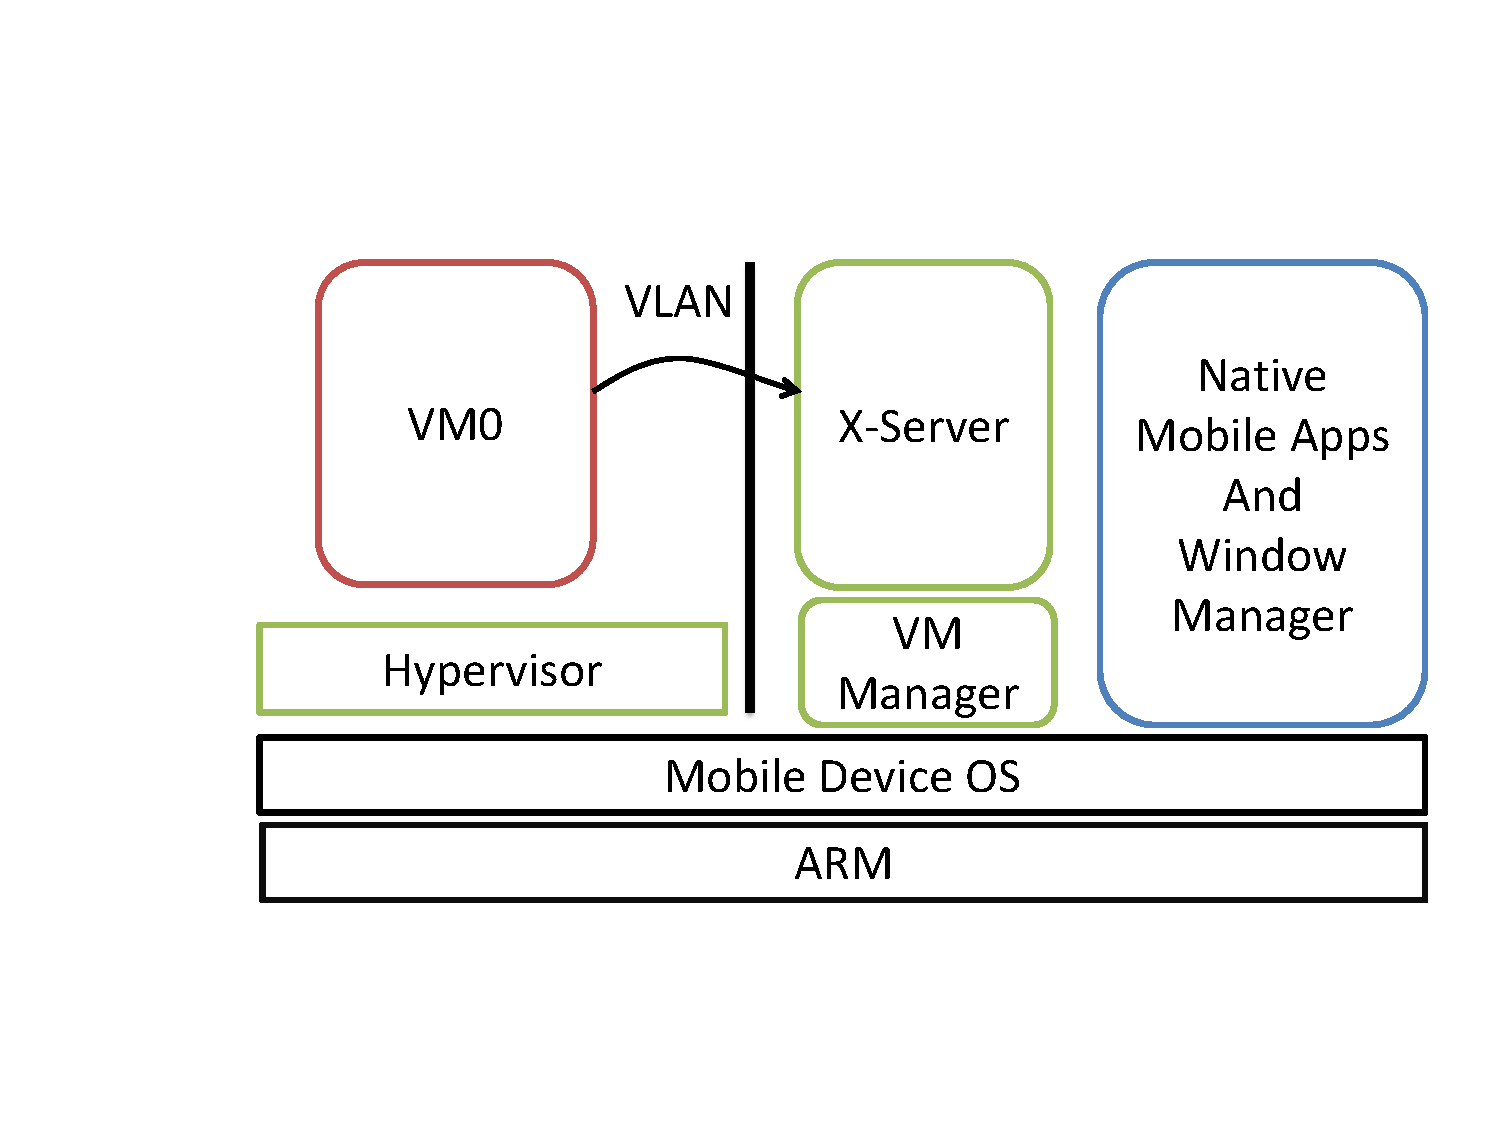
\includegraphics[width=1.0\columnwidth]{arch}
\caption{Architecture diagram}
\label{fig:arch}
\end{figure}

{\bf NOTE: Add some discussion about power usage, memory constraints ? \newline}
{\bf NOTE: Explicitly state the security model \newline}

\subsection{Proposed Architecture}
\label{sec:proposedarch}
%Here describe what we propose to do, perhaps?
%Our timeline/evaluation are kinda worthless without it.
Our proposed architecture has two main components: the virtualization framework, and the integration front-end.  The virtualzation framework contains the hypervisor (QEMU or KVM based) as well as each of the spawned VM's (see Figure \ref{fig:arch}.  Each VM will contain a thin OS with the primary goal of each VM running an application.  We chose to run x86-based Operating Systems in the VM to enable a more diverse set of target applications to be run. Each of the VM's will headless themselves, but will run their applications via X, connecting to the native X server. \\

The other component is the integration front-end.  This contains a light X server that has been integrated into the host OS, and also contains the VM manager.  The VM manager will either run inside the X-server as a native application (ARM-based), or as a separate application within the host OS.  The VM manager will be the user interface that controls launching, suspending, resuming, migrating the VM's as well as ensuring the X-server is running properly. Note that most of this actual logic and functionality will be implemented by the hypervisor in the virtualization framework.\\

The shared X-server allows us to make the graphical part of the applications common, which we believe is an improvement over having each of the VM's run an X-server, and having another layer compositing those into what the user sees. Additionally the X-server will be running native code, which we hope will allow for it to be less cpu-intensive than it might otherwise. \\

Additionally we aim to have the virtualization framework be device independent, which is important because we anticipate this to be the more complex component.  The integration front-end will have to be ported for each new device we support, but we hope to make that as simple as possible.  As an example, we should be able to take advantage of existing desktop X servers and support desktops as a client for our system, but we leave that as future work.  Our first implementation will focus on one particular device and OS, but even there we will be able to support live migration of applications. \\

In summary, we propose to build a secure, usable and portable framework for mobile device virtualization. We believe our security model to be an effective method of isolatng applications and find that our design ideas are similar to other recent efforts \cite{grier2008secure} in isolating untrusted code.
